\chapter{Исследовательская часть}

\section{Технические характеристики}

Технические характеристики устройства, на котором выполнялось тестирование:

\begin{itemize}
	\item операционная система: Windows 10;
	\item оперативная память: 16 Гб;
	\item процессор: Intel® Core™ i5-8259U;
	\item количество ядер: 4;
	\item количество логических процессоров: 8.
\end{itemize}

Во время тестирования ноутбук был включен в сеть питания и нагружен только встроенными приложениями окружения и системой тестирования.

\section{Пример работы программы}
На рисунке \ref{fig:work_example} приведен пример работы программы.
\clearpage
\begin{figure}[h!]
	
	\centering{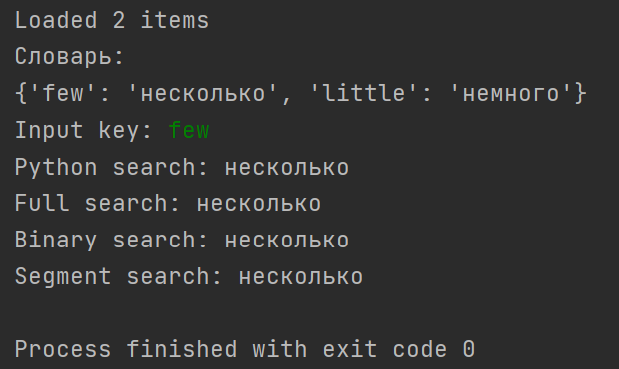
\includegraphics[scale=1]{inc/img/work_example.png}}
	
	\caption{Пример работы программы}
	
	\label{fig:work_example}
	
\end{figure}


\section{Количество сравнений}

На рисунках \ref{img:full_k}-\ref{img:segment_kg} приведены гистограммы с количеством сравнений (ось y), которые потребовались рассматриваемым реализациям алгоритмов поиска по ключам в словаре для того, чтобы найти нужный ключ (ось x). Все замеры производились в случае словаря, состоящего из 31 элемента. Для каждой реализации приведены две гистограммы, построенные по одним и тем же данным, но в первой ключи на оси x расположены в том порядке, в котором они хранились в словаре, а во второй -- упорядочены по убыванию потребовавшегося количества сравнений.

\clearpage
\img{120mm}{full_k}{Количество сравнений: полный перебор, сортировка по расположению}
\img{120mm}{full_kg}{Количество сравнений: полный перебор, сортировка по сравнениям}

\clearpage
\img{120mm}{binary_k}{Количество сравнений: бинарный поиск, сортировка по расположению}
\img{120mm}{binary_kg}{Количество сравнений: бинарный поиск, сортировка по сравнениям}

\clearpage
\img{120mm}{segment_k}{Количество сравнений: поиск в сегментированном словаре, сортировка по расположению}
\img{120mm}{segment_kg}{Количество сравнений: поиск в сегментированном словаре, сортировка по сравнениям}

Из рисунков \ref{img:full_k} и \ref{img:full_kg} видно, что количество сравнений, необходимых для поиска данного ключа полным перебором определяется только позицией ключа в словаре и равно этой позиции. Наименьшее количество сравнений (1) потребуется для самого первого ключа, наибольшее (N-количество элементов в словаре) - для последнего. Для определения того, что ключа нет в словаре, потребуется столько же сравнений, сколько и для худшего случая.

Из рисунков \ref{img:binary_k} и \ref{img:binary_kg} видно, что количество сравнений, необходимых для поиска данного ключа бинарным поиском также определяется позицией ключа в словаре, но здесь зависимость более сложная, так как надо учитывать еще и ход разбиения исходного словаря. Наименьшее количество сравнений (1) потребуется для серединного ключа, далее 2 сравнения для элементов на границе 1/4 и 3/4, а наибольшее - $(2*\log{N+1}) - 1$ (в данном примере для нечетных). Для определения того, что ключа нет в словаре, потребуется столько же сравнений, сколько и для худшего случая.

Из рисунков \ref{img:segment_k} и \ref{img:segment_kg} видно, что количество сравнений, необходимых для поиска данного ключа в сегментированном словаре определяется не только позицией ключа в своем сегменте, но и размером этого сегмента (так как наибольшие сегменты размещены ближе к началу). Наименьшее количество сравнений (2) потребуется для поиска самого первого ключа в самом большом сегмента, а наибольшее в общем случае определить нельзя: таковым может оказаться, например, ключ на <<неудачной>> позиции в самом большом сегменте или единственный ключ из самого маленького сегмента. Для определения того, что ключа нет в словаре потребуется столько же сравнений, сколько сегментов в словаре, если других ключей, начинающихся на ту же букву нет, а в противном случае -- сумма сравнений для нахождения потенциально подходящего сегмента и определения, что в нем нет искомого ключа.



Таким образом, в общем случае наибольшее количество сравнений требуется в алгоритме полного перебора. Соотношение количества сравнений в бинарном поиске и поиске в сегментированном словаре определяется размером словаря и количеством и размером сегментов в сегментированном словаре.

\clearpage
\section{Сравнение трудоемкостей реализаций}

Рассмотрим трудоемкости алгоритмов при словаре с N ключами.

\begin{itemize}
	\item Поиск полным перебором
	\begin{itemize}
		\item Трудоемкость в среднем может быть рассчитана как математическое ожидание по формуле (\ref{for:brute}), где $\Omega$ -- множество всех возможных случаев.
		
		\begin{equation}
			\label{for:brute}
			\begin{aligned}
				\sum\limits_{i \in \Omega} p_i \cdot f_i = \frac{1}{N + 1} \cdot ((\sum\limits_{i \in [1, N]}i) + N) = \\
				= \frac{1}{N + 1} \cdot (\frac{1 + N}{2} \cdot N + N) \sim \frac{N}{2} + 1
			\end{aligned}
		\end{equation}
			
		%\begin{equation}
		%\label{for:brute}
		%\begin{aligned}
			%\sum\limits_{i \in \Omega} p_i \cdot f_i = & (k_0 + k_1) \cdot \frac{1}{N + 1} + (k_0 + 2 \cdot k_1) \cdot \frac{1}{N+1} +\\
		%	& + (k_0 + 3 \cdot k_1) \cdot \frac{1}{N + 1} + (k_0 + Nk_1)\frac{1}{N + 1} + (k_0 + N \cdot k_1) \cdot \frac{1}{N + 1} =\\
		%& = k_0\frac{N+1}{N+1}+k_1+\frac{1 + 2 + \cdots + N + N}{N + 1} = \\
			%& = k_0 + k_1 \cdot \left(\frac{N}{N + 1} + \frac{N}{2}\right) = k_0 + k_1 \cdot \left(1 + \frac{N}{2} - \frac{1}{N + 1}\right)
		%\end{aligned}
	%\end{equation}
		
		\item Лучший случай - когда ключ стоит на первой позиции в словаре, и тогда придется сравнить искомый ключ только один раз, а трудоемскость составит O(1).
		
		\item Худший случай - когда ключ стоит на последней позиции в словаре, и тогда придется сравнить искомый ключ с каждым ключом словаря, а трудоемскость составит O(n).
		
		\item Добавлять новый элемент в словарь можно на любую позицию, трудоемкость добваления O(1).

	\end{itemize}


	\item Бинарный поиск
	\begin{itemize}
	\item Трудоемкость в среднем составляет $O(\log{N})$~\cite{second_article}.
	
	\item Лучший случай - когда ключ стоит на серединной позиции в словаре, и тогда придется сравнить искомый ключ только один раз, а трудоемскость составит O(1).
	
	\item Худший случай - когда ключ стоит на такой позиции, что исходный словарь придется разбивать на части вплоть до того момента, когда левая и правая границы поиска совпадут. Тогда придется сравнить искомый ключ с каждым ключом словаря $(2*\log{N+1}) - 1$ раз и трудоемскость составит $O(\log{N})$.
	
	\item Добавлять новый элемент в словарь нужно так, чтобы он остался отсортированным, трудоемкость добваления O(N).
	
	\end{itemize}


	\item Поиск в сегментированном словаре

\end{itemize}

Трудоемкость определения того, что заданный ключ отсутсвтует в словаре в каждом алгоритме равна трудоемкости худшего случая


Средняя трудоёмкость при множестве всех возможных случаев $\Omega$ может быть рассчитана по формуле (\ref{for:anal}). 

\begin{equation}
	\label{for:anal}
	\sum_{i \in \Omega}{\left(f_{\text{выбор сегмента i-ого элемента}} + f_{\text{бинарный поиск i-ого элемента}}\right)} \cdot p_i
\end{equation}

Возможны два случая определения отсутсвия ключа в словаре. Если в словаре нет ключей, начинающихся на ту же букву, то поиск значения по ключу закончится на этапе поиска нужного сегмента. Иначе понадобится осуществить еще и поиск внутри сегмента.

трудоемкость пополнения словаря


\section{Сравнение времени выполнения реализаций алгоритмов}

Сравнивалось процессорное время работы реализаций алгоритмов поиска в словаре по ключу: алгоритма полного перебора, алогоитма бинарного поиска и алгоритма поиска в сегментированном словаре. Эти реализации сравнивались по времени работы при количестве ключей в словаре 100, 1000, 5000, 10000 и 40000.

Для каждого алгоритма и каждого количества заявок проводилось 2 замера времени. Первый был связан с поиском ключей, которые на самом деле есть в словаре, причем осуществлялся поиск каждого ключа, что позволило сымитировать равновозможность выбора ключа. Второй замер связан с поиском ключей, которых на самом деле нет в словаре. Таких <<несуществующих>> ключей генерировалось столько, сколько всего ключей было в словаре.
 
Так как некоторые задачи выполняются достаточно быстро, а замеры времени имеют некоторую погрешность, они для каждой реализации, каждого объема словаря и каждого ключа выполнялись 10 раз, а затем вычислялось среднее время работы.
 

На рисунке \ref{img:time_all} приведены результаты сравнения времени выполнения реализаций алгоритмов. На графике введены следующие обозначения: full\_x - алгоритм полного перебора, binary\_x - алгоритм бинарного поиска, segment\_x - алгоритм поиска в сегментированном словаре, x=e (exists) - время работы соответсвующего алгоритма при поиске существующих ключей, x=n (not exist) -- при поиске несуществующих ключей.

\clearpage
\img{120mm}{time_all}{Сравнение времени работы реализаций в зависимости от объема словаря}

Как видно из графиков, для поиска существующего ключа наибольшее количество процессорного времени требуется алгоритму полного перебора, наименьшее - поиску в сегментированном словаре. Для определения того, что в словаре нет заданного ключа, наибольшее количество процессорного времени требуется опять же алгоритму полного перебора, наименьшее - бинарному поиску. Это различие в <<наилучшем>> алгоритме появляется в результате того, что при поиске несуществующего ключа в сегментированном словаре на бинарный поиск, являющийся его частью, накладывается еще и поиск нужного сегмента.

С увеличением размеров словаря разница во времени работы алгоритмов увеличивается.

Однако необходимо учитывать, что в случае бинарного поиска может понадобиться время на предварительную сортировку словаря, а в случае поиска в сегментированном словаре - на саму сегментацию словаря и сортировку значений внутри сегментов.


%Также можно отметить тот факт, что при использовании алгоритма бинарного поиска и поиска в сегментированном словаре, время поиска существующего ключа меньше времени определения отсутсвия заданного ключа 




\clearpage
\section{Вывод из исследовательской части}

Таким образом, в ситуациях, когда количество городов велико (более 8, например), а задача коммивояжера не требует абсолютно точного ответа, для ее решения можно использовать муравьиный алгоритм вместо алгоритма полного перебора, что позволит сэкономить процессорное время. При этом заранее проведенная параметризация может помочь настроить первый алгоритм так, что и он будет в большинстве случаев выдавать точный ответ. 

При небольшом же размере графа (прмерно до размерности 8х8) муравьиный алгоритм с большой вероятностью даст точный ответ, однако в этом случае он не дает выигрыша по времени перед алгортмом полного перебора.